\documentclass[10pt]{article}
\DeclareUnicodeCharacter{2212}{-}
\DeclareUnicodeCharacter{202C}{}
\usepackage{fancyhdr}
\usepackage{listings}
\usepackage{amsmath}
\usepackage{graphicx}
\graphicspath{ {./images/} }
\pagestyle{fancy}
\lhead{Samuel Petit 17333946}
\rhead{Statistical Methods Final Exam}
\renewcommand{\headrulewidth}{0.4pt}
\renewcommand{\footrulewidth}{0.4pt}

\begin{document}
\section*{Question 1}
\subsection*{Part a}
We have a total of 10 topics and need to pick 3 per exam so the amount of possible combinations
is $\begin{pmatrix} 10 \\ 3 \end{pmatrix} = 120$. This works for unordered topics without replacement.


\subsection*{Part b}
There are $\begin{pmatrix} 10 - n \\ 3 \end{pmatrix}$ combinations of exams such that 
no studied topics appear. Dividing this number with the total combination of exams from 
part a gives us the probability of failing:
$\frac{\begin{pmatrix} 10 - n \\ 3 \end{pmatrix}}{120}$.


\subsection*{Part c}
It is easier to derive an expression for passing. There are 2 cases to consider. 
When 2 out of the 3 topics were studied, there are $(10 - n) * \begin{pmatrix} n \\ 2 \end{pmatrix}$
combinations. This multiplies the number of combinations for the non studied topic by the
combinations of 2 studied topics. When all 3 topics on the exam were studied, there are 
$\begin{pmatrix} n \\ 3 \end{pmatrix}$ combinations thus the probability of failing the exam is: $    1 - [ \frac{(10 - n) * \begin{pmatrix} n \\ 2 \end{pmatrix} + \begin{pmatrix} n \\ 3 \end{pmatrix}}{\begin{pmatrix} 10 \\ 3 \end{pmatrix}}]$.
The plot is provided in the following question (part d).

\subsection*{Part d}
When an exam is composed of 4 questions there are 3 cases to consider in order to obtain an expression for passing the exam.
Using the same idea from part c, we sum the amount of combinations for knowing, 2, 3 and 4 of the topics on the exam:
$1 - [\frac{\begin{pmatrix} 10 - n \\ 2 \end{pmatrix}\begin{pmatrix} n \\ 2 \end{pmatrix}+(10 - n)\begin{pmatrix} n \\ 3 \end{pmatrix} + \begin{pmatrix} n \\ 4 \end{pmatrix}}{\begin{pmatrix} 10 \\ 4 \end{pmatrix}}]$.
Using the code in the Appendix section A,  I obtained the following plot. We notice that
a 4 question exam system is easier to pass for any number of studied topics, with the biggest difference
occuring when $ n = 4 $ and $ n = 5 $ and very low chance of failing when $ n \geq 6$. For a 3 questions exam the probability
is as low when $ n \geq 8 $, making the exam much simpler to pass with a 4 question system.
\begin{center}
    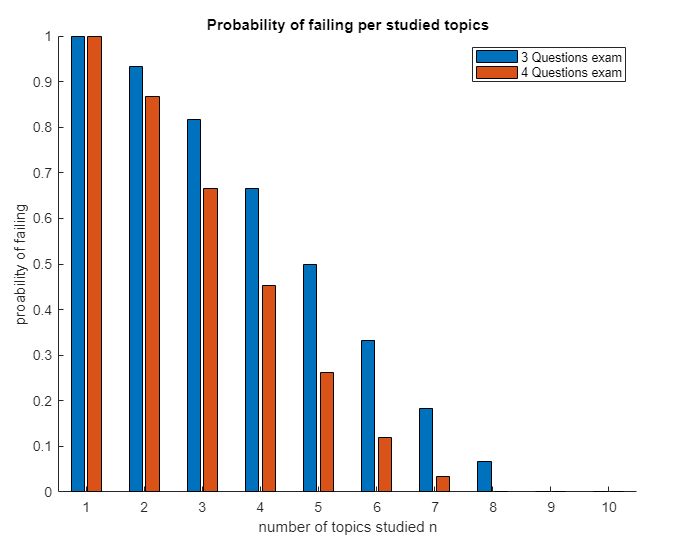
\includegraphics[scale=0.4]{final_11}
\end{center}

\subsection*{Part e}
The code for the stochastic simulation is in the appendix section B. 

\subsection*{Part f}
The code for the extended simulation is in the appendix section C.
The expression for a 95\% confidence interval using the central limit theorem is $[\mu − 1.96\sigma, \mu + 1.96\sigma]$.
Here we have $ \mu = E[X_{i}] $. So we only need to find and expression for $ \sigma $.
$ var(\frac{1}{n} \sum_{i=1}^N Y_{i}) = \frac{1}{n^2} \sum_{i=1}^N var(Y_{i}) = \frac{var(Y_{i})}{n} = \sigma^2$.
Finally, $ \sigma = \sqrt{\frac{E[X_{i}] * (1 - E[X_{i})}{N}} = \sqrt{\frac{0.1497}{N}} $. So our expression for
a 95\% confidence interval using CLT is $[E[X_{i}] − 1.96\sqrt{\frac{0.1497}{N}}, E[X_{i}] + 1.96\sqrt{\frac{0.1497}{N}}]$
Using $ N = 1000 $ and $ N = 10000 $ we then get $ [0.79272, 0.84068]_{N=1000} $ and $ [0.80912, 0.82428]_{N=10000} $ 


\subsection*{Part g}
I will use Chebyshev's inequality with 95\% confidence and solve for n to find how many times I should run
my simulation. Let's choose $\epsilon = 0.1 $ , we have $ E[X_{i}] = 0.8167 $ and $ var(X_{i}) = 0.1497$
from previous questions. Then we have: $ P(|Y - E[X_{i}| \geq 0.1) \leq \frac{0.1497}{n(0.1)^2} $
$\Leftrightarrow \frac{0.1497}{n(0.1)^2} \leq 0.05 \Leftrightarrow n \geq 299$. So I will run my simulation 300 times.
Running with $ N = 1000 $ we find that the emprical mean falls 94.3\% of the times within the interval. With 
$ N = 10000 $ it is 96.3\%. We find that both values of N fall very close to 95\%.
The CLT confidence intervals were built with with 95\% accuracy so everything is in order.

\subsection*{Part h}
If students know that topics from the previous exam are more likely to appear, we can observe that overall students
they will likely prioritise studying those topics. However this also only applies to 3 topics and thus
some students may also still decide to study potentially easier topics instead of a certain topic 
from the previous year. So in general a system like this would affect overall how the class studies but
it would not get rid of students deciding to only study different topics either. Thus I believe it makes sense to 
use the same weights for drawing the exam questions as for drawing the topics a student decides to study.
Using the simulation, We notice an overall increase in the mean of passing, with the empirical mean getting close to 
$0.5$ when $4.5$ topics are studied, and gets near $0.8$ when $6$ topics are studied. In the case that exam  
questions are less likely to appear if they were in the previous exam then with students using the same approach as 
previously outlined, except this time being less likely to study those topics, we also notice
an increase overall in means for passing for all amounts of topics studied however the difference is not as big as the previous
since this leaves $7$ remaining topics that are more likely to be drawn, so the probability for one of these to appear in the
exam would be significantly lower than previously where only 3 topics were more likely to be drawn.
Finally, if questions are excpected to be more predictable based on the previous exam when they are in fact 
chosen at random will negatively affect the mean of passing students for all amounts of studied topics. This is 
due to the fact that students will prioritise a subset of topics which are infact as likely to be drawn as 
any other topic.


\section*{Question 2}
Data id: $0.29:0.5-0.374:2-0.584:2-0$
\subsection*{Part a}
Using code provided in the appendix E, I was able to produce the following
plot.  
We notice that question 1 is very spread out and uneven in probability. We can
assume that it was very easy to obtain a grade of 100\% given that a student studied that topic.
Question 2 and 3 seem to be following student distribution.
\begin{center}
    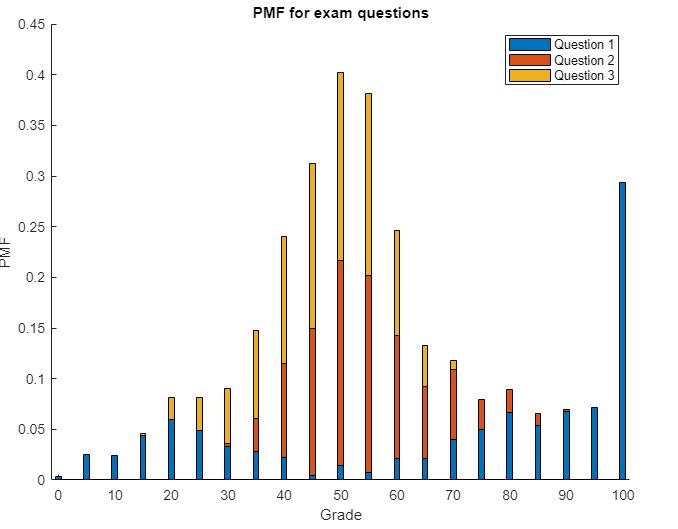
\includegraphics[scale=0.385]{final_pmf}
\end{center}
However we notice higher grades for question 2 meaning that it is probably easier.
Question 3 seem to be harder as we notice a significant probability for grades below 40\%.
This approach can be good to use as if an entire class obtains low grades, the PMF will reflect that and 
that can be a good indicator that an question is likely to be hard.
On the other hand, it could lead to false positives as students as a group are likely to study
similar topics, we could notice a low PMF for a question that was in fact easy but the students did not
study for.

\subsection*{Part b}
The code for this question is added to the appendix section F. I decided to use binnings
with a range of 10\% as it allowed for a cleaner display of means and variances while keeping 
accuracy (for instance making the ranges too wide would lose too much accuracy and thus would 
make it harder to draw conclusions).

\subsection*{Part c}
The code to obtain the following plot is also in the appendix section F as it was integrated with part b's code.
I decided to use CLT 95\% confidence intervals.
\begin{center}
    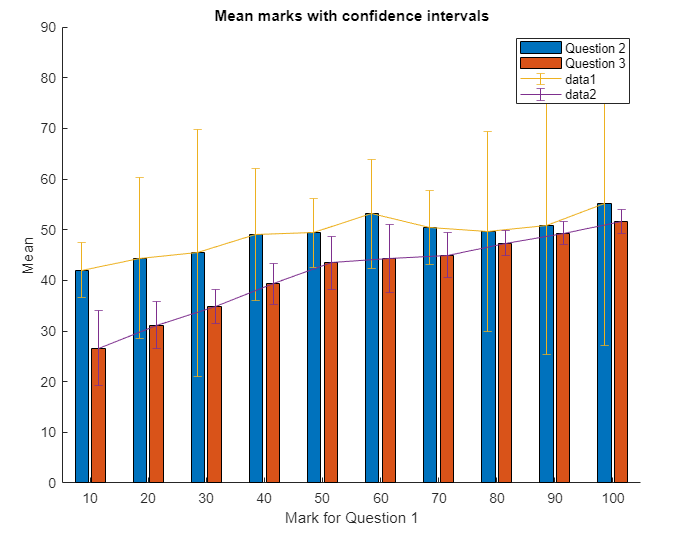
\includegraphics[scale=0.45]{final_c}
\end{center}
In question 2, we notice that the means for all categories is always above
40. We also notice that students who did poorly in question 1 obtained grades in question 2 very similar 
to students who scored relatively high in question 1. 
Using confidence intervals, we observe that students with high grades for question
1 obtained very varied scores in question 2 as the intervals are very large. 
Thus it seems question 2 is a harder question to obtain high grades in than question 1, however it seems to be 
relatively easy to obtain a score of 40\%. 
In question 3, we notice a more usual distribution with students who did poorly in question 1 getting lower grades than
those who scored well in question 1. However, we also notice once again that those who obtained high grades
in question 1 obtained a grade near 50\% for question 3 with very small confidence intervals meaning
that this question is very likely to be hard to score high in.


\subsection*{Part d}
Using the mark obtained in question 1 as an input to our model and marks for the following questions
as training data, we can use linear regression to predict marks for a student.
We would use the hypothesis $ h_{\theta}(x) = \theta_{0} + \theta_{1}x_{1} + \theta_{2}x_{2} $.
We would then measure the accuracy of our model using the following cost function 
$ J(\theta) = \frac{1}{m}\sum_{i = 1}^m (h_{\theta}(x^{i}) - y^{i})^2$. Finally, to get the most accurate
predictions, we want to find values for our parameters such that they minimize the outputs of our loss
function. One way to do this is by using gradient descent. Thus we can use the following algorithm to find such
values. Repeat the following 2 steps: Step 1 - for j=0 to n: $ tmp_{j} = \theta_{j} - \frac{2\alpha}{m}$
$\sum_{i = 1}^m (h_{\theta}(x^{(i)}) - y^{(i)})x_{j}^{(i)}$. Step 2 - for j=0 to n: $ \theta_{j} = tmp_{j} $.
According to the graph from part c, it seems that question 3 follows a linear regression. Question 2 however
is not as clear, it seems to follow a linear pattern however the confidence intervals for grades over 70\% are 
too wide to be able to make decisions on which model might be better suited, perhaps a cubic model could work better here.
The type of randomness assumed in linear regression is applicable for exam marks as many different factors
outside of previously obtained grades affect a grade, things such as fatigue, performance, stress or even lecturer grading for example.

\subsection*{Part e}
Since we know that marks $ X_{ij} $ are normally distributed 
($X_{ij}\sim N(S_{i} - D_{j}, \sigma^2)$). Then the probability density function is 
$ \frac{1}{\sigma\sqrt{2\pi}}e^{-\frac{1}{2}(\frac{x - (S_{i} - D_{j})}{\sigma})^2} $.
Finally, given that all student marks are independent we can use this PDF to obtain a 
log-likelihood function. $ \prod_{i = 1}^N\frac{1}{\sigma\sqrt{2\pi}} e^{-\frac{(x - S_{i} - D_{j})^2}{2\sigma^2}} $
$ = (\sigma^{2}2\pi)^{-N/2}e^{-\frac{1}{2\sigma^2}\sum_{i = 1}^N(S_{i} - D_{j})^2} $.

\subsection*{Part f}
We are looking to estimate values for parameters $S_{i}, D_{j}$ such that they maximise the above log-likelihood
function. We can use gradient ascent, the algorithm is the same as part d however we will be using
the negative loss function such as to find a maximum. Thus the algorithm here is also in 2 steps.
Step 1 - for j=0 to n: $ tmp_{j} = \theta_{j} + \frac{2\alpha}{m}$
$\sum_{i = 1}^m (h_{\theta}(x^{(i)}) + y^{(i)})x_{j}^{(i)}$. 
Step 2 - for j=0 to n: $ \theta_{j} = tmp_{j} $ 
Note that in this case we have 2 unknown parameters $ \theta $, these are $ S_{i} $ and $ D_{j} $.

\section*{Appendix}
\subsection*{Section A - Question 1c and 1d}
Code to plot the probability of failing against the number of 
studied topics for both 3 and 4 questions exam types. \\
\begin{lstlisting}
y4qs = zeros([1 10]);
y3qs = zeros([1 10]);
% for all values of n
for n = 1:10
    % probability of failing for a 3 questions exam
    y3qs(n) = 1 - (((10-n) *
        (customNChooseK(n,2))/customNChooseK(10,3))+
        (customNChooseK(n,3)/customNChooseK(10,3)));
    % probability of failing for a 4 question exam
    y4qs(n) = 1 - (((10-n)*(customNChooseK(n,3)) /
        customNChooseK(10,4))+ (customNChooseK(n,4) /
        customNChooseK(10,4)) + (customNChooseK(10-n,2) *
        (customNChooseK(n,2)/customNChooseK(10,4))));
end

figure
hold on

xAxis = 1:1:10;
yAxis = [y3qs; y4qs];
xlabel('number of topics studied n')
ylabel('proability of failing')
bar(xAxis, yAxis);
legend(['3 Questions exam'; '4 Questions exam']);
title('Probability of failing per studied topics');

function [m] = customNChooseK(n,k)
    if(n < k)
        m = 0;
    else
        m = nchoosek(n,k); 
    end
end
\end{lstlisting}


\subsection*{Section B - Question 1e}
Code for a stochastic simulation of the exam setup with three questions.
Function takes a number $ n $ which designs the amount of studied topics.
The simulation picks randomly a set of studied topics and exam topics 
and returns 1 if the student passes, else 0.
\begin{lstlisting}
function [X] = simulation3Questions(n)
    % number of topics
    topics=1:10;
    % draw for exam questions
    questions = randperm(numel(topics),3);
    % draw for studied subjects
    studiedSubjects = randperm(numel(topics),n); 
    
    % get common topics
    pos=intersect(questions, studiedSubjects);
    % return 1 if pass or 0 if fail
    if(length(pos) >= 2)
        X = 1; 
    else 
        X =0;
    end
end    
\end{lstlisting}


\subsection*{Section C - Question 1f}
Extended stochastic simulation. Runs the above simulation in Section B
N times and returns the empirical mean. $\\$
\begin{lstlisting}
function [X] = simulationEmpiricalMean(n, N)
    passCount = 0;
    % run N times keeping count of amount of pass
    for i = 1:N
        % number of topics
        topics=1:10;
        % draw exam questions
        questions = randperm(numel(topics),3);
        % draw studied subjects
        studiedSubjects = randperm(numel(topics),n); 

        % get common topics
        common=intersect(questions, studiedSubjects);
        if(length(common) >= 2)
            passCount = passCount + 1;
        end 
    end
    % return empirical mean
    X = passCount / N;
end 
\end{lstlisting}

\subsection*{Section D - Question 1g}
Code for running the extended stochastic simulation N times and
displaying the percentage of times that the simulated empirical mean falls within a
confidence interval.
\begin{lstlisting}
% count for times mean falls within interval
count = 0;
% 1000 or 10000 depending on simulation to run
N = 1000;
% Amount of times to run simulation
size = 300;
% Values of the confidence interval (here for N = 1000)
lo = 0.79272;
hi = 0.84068;

% Run simulation size times and increment count if 
% the mean falls within the CI
for i = 1:size
    % function from appendix section C
    % returns the empirical mean.
    simMean = simulationEmpiricalMean(7, N);
    if(simMean >= lo && simMean <= hi)
        count = count + 1;
    end
end
% Display % of means falling within confidence interval
disp(count/size * 100);
\end{lstlisting}

\subsection*{Section E - Question 2a}
Code for running obtaining the PMF for all 3 questions from the data set
and plot the results.
\begin{lstlisting}
data = load('data.txt');
nstudents = length(data(:,1));

countsQ1=zeros(1, 101);
countsQ2=zeros(1, 101);
countsQ3=zeros(1, 101);

gradesQ1 = data(:,1);
gradesQ2 = data(:,2);
gradesQ3 = data(:,3);

% Go through all students keeping counts
% For all grades
for i=1:nstudents
    countsQ1(gradesQ1(i) + 1) = 
        countsQ1(gradesQ1(i)+ 1) + 1; 
    countsQ2(gradesQ2(i) + 1) = 
        countsQ2(gradesQ2(i)+ 1) + 1; 
    countsQ3(gradesQ3(i) + 1) = 
        countsQ3(gradesQ3(i)+ 1) + 1; 
end
figure
hold on

combined = [countsQ1/nstudents; 
    countsQ2/nstudents; countsQ3/nstudents];
bar(0:100,combined, 1,'stacked');
xlabel('Grade');
ylabel('PMF');
legend(['Question 1'; 'Question 2'; 'Question 3']);
title('PMF for exam questions');
bar(xAxis, yAxis);
    
\end{lstlisting}

\subsection*{Section F - Question 2b and 2c}
Code for calculating means, variances and confidence intervals
for question 2 and 3 conditioned on question 1.
\begin{lstlisting}
% Q2 b
m = 1000;
data = load('data.txt');
means = 1:10;
vars = 1:10;
cis=[];

% go through all 10 categories
for i = 1:10
    index=1;
    studentsInCat = zeros([1 1]);
    % go through all students and 
    % add to category if grade from q1 is in
    % the current category
    for j = 1:m
        grade = data(j, 1);
        if (grade < i*10) && grade >= (i*10)-10
            studentsInCat(index,1) = j;
            index = index + 1;
        end
    end
    
    % get list of grades from all 
    % students who fall in the category
    % and their means
    nbStudents = numel(studentsInCat);
    index = 1;
    % array to contain all grades of 
    % all students for q2 and 3 from the
    % current category 
    grades = 1:2*nbStudents;
    for cQuestion = 2:3
        gradeSum = 0;
        for cStudent = 1:nbStudents       
            grade = data(studentsInCat(cStudent)
                ,cQuestion);
            grades(index) = grade;
            index = index + 1;
            gradeSum = gradeSum + grade;
        end
        
        % keep variance and mean for 
        % current question / bracket
        vars(i,cQuestion-1) = var(grades);
        means(i,cQuestion-1) = gradeSum/nbStudents;
        
        % 2c - Compute confidence interval
        % Using CLT
        stdDev = sqrt(vars(i,cQuestion-1))
            /sqrt(nbStudents);
        cis(i,cQuestion-1,1) = means(i)-(2*stdDev);
        cis(i,cQuestion-1,2) = means(i)+(2*stdDev);
    end 
end

figure
hold on

% plot means for both questions & all 10 categories
xaxis = 10:10:100;
yaxis = [reshape(means(:,1),1,10);
    reshape(means(:,2),1,10)];
xlabel('Mark for Question 1');
ylabel('Mean');
title('Mean marks with confidence intervals');
bar(xaxis, yaxis);

errq1 = ones(10,1);
errq2 = ones(10,1);

% get difference between high and lower bound as error
for i = 1:10
    errq1(i) = cis(i,1,2) - cis(i,1,1);
    errq2(i) = cis(i,2,2) - cis(i,2,1);
end

% plot error bars
legend({'Question 2','Question 3'})
errorbar(xaxis - 1.5,reshape(means(:,1),1,10), errq1);
errorbar(xaxis + 1.5,reshape(means(:,2),1,10), errq2);
\end{lstlisting}


\end{document}